\documentclass[11pt,a4paper]{article}

\usepackage[utf8]{inputenc}
\usepackage[T1]{fontenc}
\usepackage[spanish,es-nodecimaldot]{babel}
\usepackage{geometry}
\usepackage{amsmath}
\usepackage{amssymb}
\usepackage{booktabs}
\usepackage{array}
\usepackage{graphicx}
\usepackage{float}
\usepackage{hyperref}
\usepackage{tabularx}
\usepackage{enumitem}
\usepackage{xcolor}
\usepackage{caption}
\usepackage{natbib}
\usepackage{multirow}
\usepackage{url}

\geometry{margin=2.5cm}
\emergencystretch=1.5em
\hypersetup{
    colorlinks=true,
    linkcolor=blue!50!black,
    citecolor=blue!50!black,
    urlcolor=blue!50!black,
    pdftitle={Guia didactica del proyecto TD3 para protesis mioelectrica},
    pdfauthor={Proyecto EMG Prosthesis TD3}
}

\newcolumntype{L}[1]{>{\raggedright\arraybackslash}p{#1}}
\newcolumntype{C}[1]{>{\centering\arraybackslash}p{#1}}
\newcolumntype{Y}{>{\raggedright\arraybackslash}X}

\title{\textbf{Gu\'ia Did\'actica del Proyecto TD3 para una Pr\'otesis Mioel\'ectrica}\\
\large Conceptos, par\'ametros, f\'ormulas, errores encontrados y estado actual del proyecto}
\author{Proyecto \texttt{EMG\_Prosthesis\_TD3}}
\date{23 de marzo de 2026}

\begin{document}

\maketitle

\begin{abstract}
Este documento es una gu\'ia did\'actica del proyecto de control continuo de una pr\'otesis mioel\'ectrica con Twin Delayed Deep Deterministic Policy Gradient (TD3). El objetivo es explicar, de forma amplia y pedag\'ogica, qu\'e est\'a resolviendo el proyecto, c\'omo est\'a organizado el pipeline, qu\'e significa cada t\'ermino importante, por qu\'e se eligi\'o TD3, c\'omo evolucion\'o la funci\'on de recompensa desde una versi\'on heredada hasta la formulaci\'on actual basada en tracking MSE, y por qu\'e el hallazgo de un bug en el simulador cambi\'o la interpretaci\'on de varias corridas previas. Tambi\'en se explican las f\'ormulas principales del estado, la reward y el remapeo de acci\'on, adem\'as de la lectura correcta de las gr\'aficas de entrenamiento y de los tests visuales. La gu\'ia termina con una interpretaci\'on clara del baseline v\'alido actual, obtenido con una corrida de 8000 episodios y el checkpoint \texttt{Agent7250}, que hoy representa la mejor versi\'on defendible del proyecto en simulaci\'on.
\end{abstract}

\tableofcontents
\newpage

\section{Para qu\'e sirve esta gu\'ia}

Esta gu\'ia no pretende reemplazar el reporte t\'ecnico del proyecto. Su funci\'on es distinta: servir como documento de estudio para entender qu\'e se hizo, por qu\'e se hizo y c\'omo interpretar el sistema actual. Por eso el texto tiene un tono m\'as pedag\'ogico que de art\'iculo experimental.

En particular, la gu\'ia intenta responder preguntas como:
\begin{itemize}[leftmargin=1.2cm]
    \item \emph{Qu\'e problema resuelve exactamente este proyecto?}
    \item \emph{Por qu\'e se usa TD3 y no otro algoritmo?}
    \item \emph{Qu\'e significa reward shaping en este contexto?}
    \item \emph{Por qu\'e la reward inicial era insuficiente?}
    \item \emph{Qu\'e cambi\'o al pasar a una reward basada en MSE?}
    \item \emph{Qu\'e fue el bug del simulador y por qu\'e fue tan importante?}
    \item \emph{C\'omo se interpreta el baseline actual de 8000 episodios?}
\end{itemize}

\section{Qu\'e problema resuelve el proyecto}

El proyecto busca controlar una pr\'otesis rob\'otica de mano a partir de se\~nales EMG. El objetivo no es solo clasificar gestos discretos, sino lograr una operaci\'on continua, es decir, que la pr\'otesis pueda modular su movimiento de forma proporcional y no binaria. Esa idea est\'a alineada con el art\'iculo base del proyecto \citep{fuertes2026continuous} y con la literatura de control mioel\'ectrico reciente \citep{chen2023review}.

En t\'erminos simples:
\begin{itemize}[leftmargin=1.2cm]
    \item la persona activa ciertos grupos musculares;
    \item esas activaciones se registran como EMG;
    \item el agente TD3 recibe una representaci\'on de esa EMG;
    \item el agente decide una acci\'on continua para cuatro motores;
    \item la pr\'otesis se mueve;
    \item el sistema mide qu\'e tan cerca qued\'o respecto a una referencia deseada.
\end{itemize}

\section{Pipeline general del sistema}

La forma m\'as simple de entender el proyecto es mediante el pipeline de aprendizaje por refuerzo:
\begin{equation}
\text{EMG/observaciones}
\rightarrow
\text{estado}
\rightarrow
\text{actor TD3}
\rightarrow
\text{acci\'on}
\rightarrow
\text{entorno}
\rightarrow
\text{reward}
\rightarrow
\text{buffer}
\rightarrow
\text{actualizaci\'on TD3}.
\end{equation}

En este proyecto, ese pipeline se materializa as\'i:
\begin{enumerate}[leftmargin=1.2cm]
    \item se calcula un vector de 40 features EMG;
    \item se a\~nade realimentaci\'on del estado mec\'anico de la pr\'otesis;
    \item el actor de TD3 produce cuatro acciones continuas en \([-1,1]\);
    \item el entorno remapea esas acciones a PWM efectivos;
    \item el simulador actualiza la posici\'on de la pr\'otesis;
    \item se calcula una reward basada en tracking y regularizaci\'on;
    \item la transici\'on se almacena en replay buffer;
    \item actor y cr\'iticos se actualizan seg\'un las reglas de TD3 \citep{fujimoto2018td3,mathworks_td3_agent,mathworks_td3_options}.
\end{enumerate}

\section{Glosario de t\'erminos clave}

\subsection{EMG}

EMG significa electromiograf\'ia. En este proyecto, la EMG representa la actividad muscular del antebrazo y sirve como proxy de la intenci\'on motora del usuario.

\subsection{Features EMG}

No se alimenta la red con la se\~nal cruda. En lugar de eso, se calculan cinco features por cada uno de ocho canales, para un total de 40 dimensiones. Esto reduce ruido y hace el estado m\'as estructurado.

\subsection{Estado u observaci\'on}

Es el vector que ve el agente en cada paso. Hoy el estado v\'alido del proyecto tiene 52 dimensiones y combina EMG actual, encoders, delta de encoders y acci\'on efectiva previa.

\subsection{Acci\'on}

Es la salida del actor. En este proyecto son cuatro valores continuos, uno por motor, acotados en \([-1,1]\).

\subsection{PWM}

PWM es la forma efectiva en que se manda la se\~nal a los motores. Aunque el actor produce valores continuos, el simulador usa niveles efectivos discretos de PWM.

\subsection{Reward}

Es la se\~nal escalar que dice al agente si una acci\'on fue mejor o peor. No es exactamente ``\'exito'' o ``fracaso'', sino una medida de cu\'an deseable fue la transici\'on.

\subsection{Reward shaping}

Es el dise\~no de esa reward para que el agente aprenda el comportamiento correcto. Es uno de los puntos m\'as delicados del proyecto \citep{deng2025reward}.

\subsection{Actor}

Es la red que decide la acci\'on.

\subsection{Cr\'itico}

Es la red que estima qu\'e tan buena es una acci\'on en un estado dado. TD3 usa dos cr\'iticos para reducir sobreestimaci\'on \citep{fujimoto2018td3}.

\subsection{Replay buffer}

Es una memoria donde se guardan experiencias pasadas para entrenar de forma m\'as estable y menos correlacionada.

\subsection{Tracking MSE}

Es el error cuadr\'atico medio entre la trayectoria de referencia y la trayectoria de la pr\'otesis. Hoy es la m\'etrica principal del proyecto.

\subsection{Tracking MAE}

Es el error absoluto medio. Es m\'as f\'acil de interpretar, pero penaliza menos los errores grandes que MSE.

\subsection{ActionL2}

Mide qu\'e tan grande es, en promedio, la magnitud de la acci\'on. Es una medida de esfuerzo de control.

\subsection{Saturation fraction}

Mide qu\'e fracci\'on de acciones efectivas cae cerca del l\'imite del actuador. Si esta m\'etrica es muy alta, el agente est\'a empujando demasiado tiempo al borde.

\subsection{\(\Delta a\) L2}

Mide qu\'e tanto cambia la acci\'on entre un paso y el siguiente. Es una medida de brusquedad o suavidad.

\subsection{Checkpoint}

Es un agente guardado durante entrenamiento. El mejor agente no siempre es el \'ultimo; por eso se auditan checkpoints.

\section{Por qu\'e se eligi\'o TD3}

TD3 se eligi\'o porque este proyecto es un problema de control continuo. El agente necesita producir acciones reales, no clases discretas. TD3 es adecuado para ese tipo de tareas porque combina tres ideas importantes \citep{fujimoto2018td3,mathworks_td3_agent}:
\begin{enumerate}[leftmargin=1.2cm]
    \item dos cr\'iticos para reducir sobreestimaci\'on;
    \item actualizaci\'on retrasada del actor para estabilizar aprendizaje;
    \item suavizado de la pol\'itica objetivo para evitar soluciones demasiado fr\'agiles.
\end{enumerate}

De forma intuitiva:
\begin{itemize}[leftmargin=1.2cm]
    \item DDPG puro puede volverse optimista de forma artificial;
    \item TD3 corrige parte de ese optimismo;
    \item eso lo vuelve especialmente atractivo para control continuo con ruido y estados complejos.
\end{itemize}

\section{C\'omo evolucion\'o la reward}

\subsection{Reward heredada inicial}

La reward heredada intentaba combinar varias ideas a la vez:
\begin{itemize}[leftmargin=1.2cm]
    \item premiar direcci\'on correcta;
    \item castigar movimiento inverso;
    \item incentivar no quedarse quieto;
    \item penalizar distancia respecto a la referencia;
    \item penalizar cambios bruscos.
\end{itemize}

En teor\'ia, eso suena razonable. En la pr\'actica, generaba varios problemas:
\begin{itemize}[leftmargin=1.2cm]
    \item trataba acciones continuas como si fueran discretas;
    \item mezclaba l\'ogica de direcci\'on con distancia sin una escala clara;
    \item pod\'ia inducir \emph{reward hacking};
    \item no quedaba claro qu\'e t\'ermino dominaba realmente la optimizaci\'on.
\end{itemize}

El problema central aqu\'i es metodol\'ogico: una reward que parece rica no siempre es una reward buena. Si el agente encuentra una forma de maximizarla sin mejorar el tracking real, la reward no est\'a alineada con el objetivo \citep{deng2025reward}.

\subsection{Paso a una reward basada en MSE}

La primera gran limpieza consisti\'o en pasar a una reward centrada en tracking MSE. La forma m\'as simple de esa versi\'on fue:
\begin{equation}
r_t^{\text{MSE}}
=
-
\frac{1}{4}\sum_{i=1}^{4}
\left(
e_{t,i}^{2}
+
\lambda_a \tilde{a}_{t,i}^{2}
\right),
\end{equation}
con:
\begin{equation}
e_{t,i} = \hat{y}_{t,i} - y_{t,i}.
\end{equation}

Esta reward fue mejor por tres razones:
\begin{enumerate}[leftmargin=1.2cm]
    \item el objetivo principal qued\'o claro: minimizar error de tracking;
    \item el error se volvi\'o interpretable en escala normalizada;
    \item el agente dej\'o de depender tanto de reglas discretas artificiales.
\end{enumerate}

\subsection{Reward actual}

La versi\'on vigente a\~nade suavidad expl\'icita:
\begin{equation}
r_t =
-
\frac{1}{4}\sum_{i=1}^{4}
\left(
e_{t,i}^{2}
+
\lambda_a \tilde{a}_{t,i}^{2}
+
\lambda_{\Delta a}\left(\tilde{a}_{t,i} - \tilde{a}_{t-1,i}\right)^2
\right).
\label{eq:guide-reward}
\end{equation}

La interpretaci\'on de esta f\'ormula es simple:
\begin{itemize}[leftmargin=1.2cm]
    \item \(e_{t,i}^{2}\): si el tracking es malo, la reward baja;
    \item \(\lambda_a \tilde{a}_{t,i}^{2}\): si el agente usa demasiada acci\'on, paga un costo;
    \item \(\lambda_{\Delta a}(\tilde{a}_{t,i}-\tilde{a}_{t-1,i})^2\): si el agente cambia muy bruscamente de acci\'on, tambi\'en paga un costo.
\end{itemize}

Esto es importante porque el proyecto ya no busca solo que la pr\'otesis llegue al objetivo. Busca llegar bien, sin gastar acci\'on arbitrariamente ni generar trayectorias violentas.

\section{Estado actual del problema y por qu\'e tiene 52 dimensiones}

La observaci\'on actual es:
\begin{equation}
s_t =
\begin{bmatrix}
\phi_t \\
\mathrm{enc}_t \\
\Delta \mathrm{enc}_t \\
\tilde{a}_{t-1}
\end{bmatrix}
\in \mathbb{R}^{52}.
\label{eq:guide-state}
\end{equation}

Esta f\'ormula merece explicarse con calma:
\begin{itemize}[leftmargin=1.2cm]
    \item \(\phi_t\): resume la actividad EMG actual;
    \item \(\mathrm{enc}_t\): le dice al agente en qu\'e posici\'on est\'a la pr\'otesis;
    \item \(\Delta \mathrm{enc}_t\): le dice si se est\'a moviendo y en qu\'e direcci\'on;
    \item \(\tilde{a}_{t-1}\): le recuerda qu\'e acci\'on efectiva aplic\'o justo antes.
\end{itemize}

La idea intuitiva es esta: si el agente solo ve EMG actual, le falta contexto motor. Si adem\'as ve encoder, cambio de encoder y acci\'on previa, puede razonar mejor sobre la transici\'on actual.

\section{Por qu\'e se remapea la acci\'on a PWM efectivo}

Aunque el actor produce acciones continuas, el sistema no aplica cualquier valor arbitrario al motor. El entorno remapea a niveles efectivos:
\begin{equation}
\mathcal{U}_{\mathrm{PWM}} = \{0, 64, 96, 128, 160, 192, 224, 255\}.
\end{equation}

Esto se hizo porque, en la pr\'actica, el simulador y el actuador no distinguen bien valores muy peque\~nos. Si el agente aprendiera acciones continuas min\'usculas, el aprendizaje parecer\'ia correcto en matem\'aticas pero no mover\'ia realmente la pr\'otesis.

Este punto es muy importante para entender el proyecto: no basta con que la red ``quiera'' mover. Hay que alinear esa voluntad num\'erica con una acci\'on f\'isicamente efectiva.

\section{El bug del simulador explicado de forma sencilla}

\subsection{Versi\'on corta}

Durante bastante tiempo, el proyecto parec\'ia entrenar agentes, pero el simulador en realidad no estaba moviendo la pr\'otesis como deb\'ia.

\subsection{Qu\'e pasaba exactamente}

El simulador principal usaba datos de trayectoria desde \texttt{fit\_C2.mat}. El problema fue que esas trayectorias estaban vac\'ias. Entonces, aunque el agente mandara acci\'on, la pr\'otesis se quedaba casi constante.

Adem\'as, dentro de \texttt{step}, la acci\'on se reflejaba con un desfase de un paso. Eso significa que el agente actuaba en \(t\), pero el entorno parec\'ia responder en \(t+1\).

\subsection{Por qu\'e eso fue tan grave}

Porque cambia la interpretaci\'on de todo:
\begin{itemize}[leftmargin=1.2cm]
    \item si el entorno no se mueve, no se puede concluir seriamente si la reward es buena o mala;
    \item tampoco se puede concluir seriamente si 52D, 132D o LSTM mejoran o empeoran;
    \item las corridas pre-fix sirven como aprendizaje de ingenier\'ia, pero no como benchmark principal.
\end{itemize}

\subsection{C\'omo se arregl\'o}

Se hicieron dos cambios:
\begin{enumerate}[leftmargin=1.2cm]
    \item cuando \texttt{ws} est\'a vac\'io, el simulador usa \texttt{pattern\_curve.mat} como respaldo;
    \item el tiempo del episodio se adelanta antes de leer la pr\'otesis, para que la acci\'on afecte el paso actual.
\end{enumerate}

La versi\'on simple de la conclusi\'on es: antes el agente aprend\'ia en un mundo parcialmente roto; despu\'es del fix, empez\'o a aprender en un entorno f\'isicamente coherente.

\section{C\'omo leer las gr\'aficas de entrenamiento}

La ventana de entrenamiento de MATLAB muestra tres curvas importantes \citep{mathworks_train_agents,mathworks_training_options}:
\begin{itemize}[leftmargin=1.2cm]
    \item \textbf{EpisodeReward}: la recompensa total de cada episodio individual;
    \item \textbf{AverageReward}: promedio m\'ovil del reward, \'util para ver tendencia;
    \item \textbf{EpisodeQ0}: estimaci\'on del retorno esperable al inicio del episodio seg\'un el cr\'itico.
\end{itemize}

\subsection{Qu\'e significa que la reward sea negativa}

No significa necesariamente que el entrenamiento est\'e mal. En este proyecto la reward est\'a formulada como costo negativo:
\begin{equation}
r_t \le 0.
\end{equation}

Por tanto, mejorar significa acercarse a cero, no necesariamente volverse positivo.

\subsection{Qu\'e buscar en la gr\'afica}

Se busca:
\begin{itemize}[leftmargin=1.2cm]
    \item que \texttt{AverageReward} suba de forma sostenida;
    \item que \texttt{EpisodeReward} siga siendo ruidosa, pero con mejor centro;
    \item que \texttt{EpisodeQ0} no se separe de forma absurda del reward observado.
\end{itemize}

\section{C\'omo leer un test visual}

En los plots por episodio del proyecto:
\begin{itemize}[leftmargin=1.2cm]
    \item la l\'inea naranja es la referencia;
    \item la l\'inea azul es la respuesta de la pr\'otesis;
    \item las acciones anotadas muestran qu\'e est\'a mandando el agente.
\end{itemize}

La pregunta central no es solo \emph{si la azul llega}, sino:
\begin{itemize}[leftmargin=1.2cm]
    \item si acompa\~na de forma progresiva la referencia;
    \item si evita quedarse plana;
    \item si lo logra sin saturarse demasiado tiempo.
\end{itemize}

\section{El baseline v\'alido actual}

\subsection{Primera versi\'on v\'alida: 2000 episodios}

Tras el fix del simulador, la primera corrida v\'alida produjo un test con:
\begin{itemize}[leftmargin=1.2cm]
    \item \texttt{trackingMSE = 0.052805},
    \item \texttt{trackingMAE = 0.179093},
    \item \texttt{actionL2 = 0.674957},
    \item \texttt{saturationFraction = 0.474999},
    \item \(\Delta a\) L2 \(= 0.633264\).
\end{itemize}

Ese resultado fue importante porque por primera vez demostr\'o tracking real.

\subsection{Versi\'on refinada: 8000 episodios}

La corrida larga de 8000 episodios refin\'o el baseline. El mejor checkpoint auditado result\'o ser \texttt{Agent7250}, no \texttt{Agent8000}. Ese detalle es muy importante: en RL, el mejor modelo no siempre es el \'ultimo.

\IfFileExists{figures/training_progress_8000eps_valid_baseline.png}{
\begin{figure}[H]
\centering
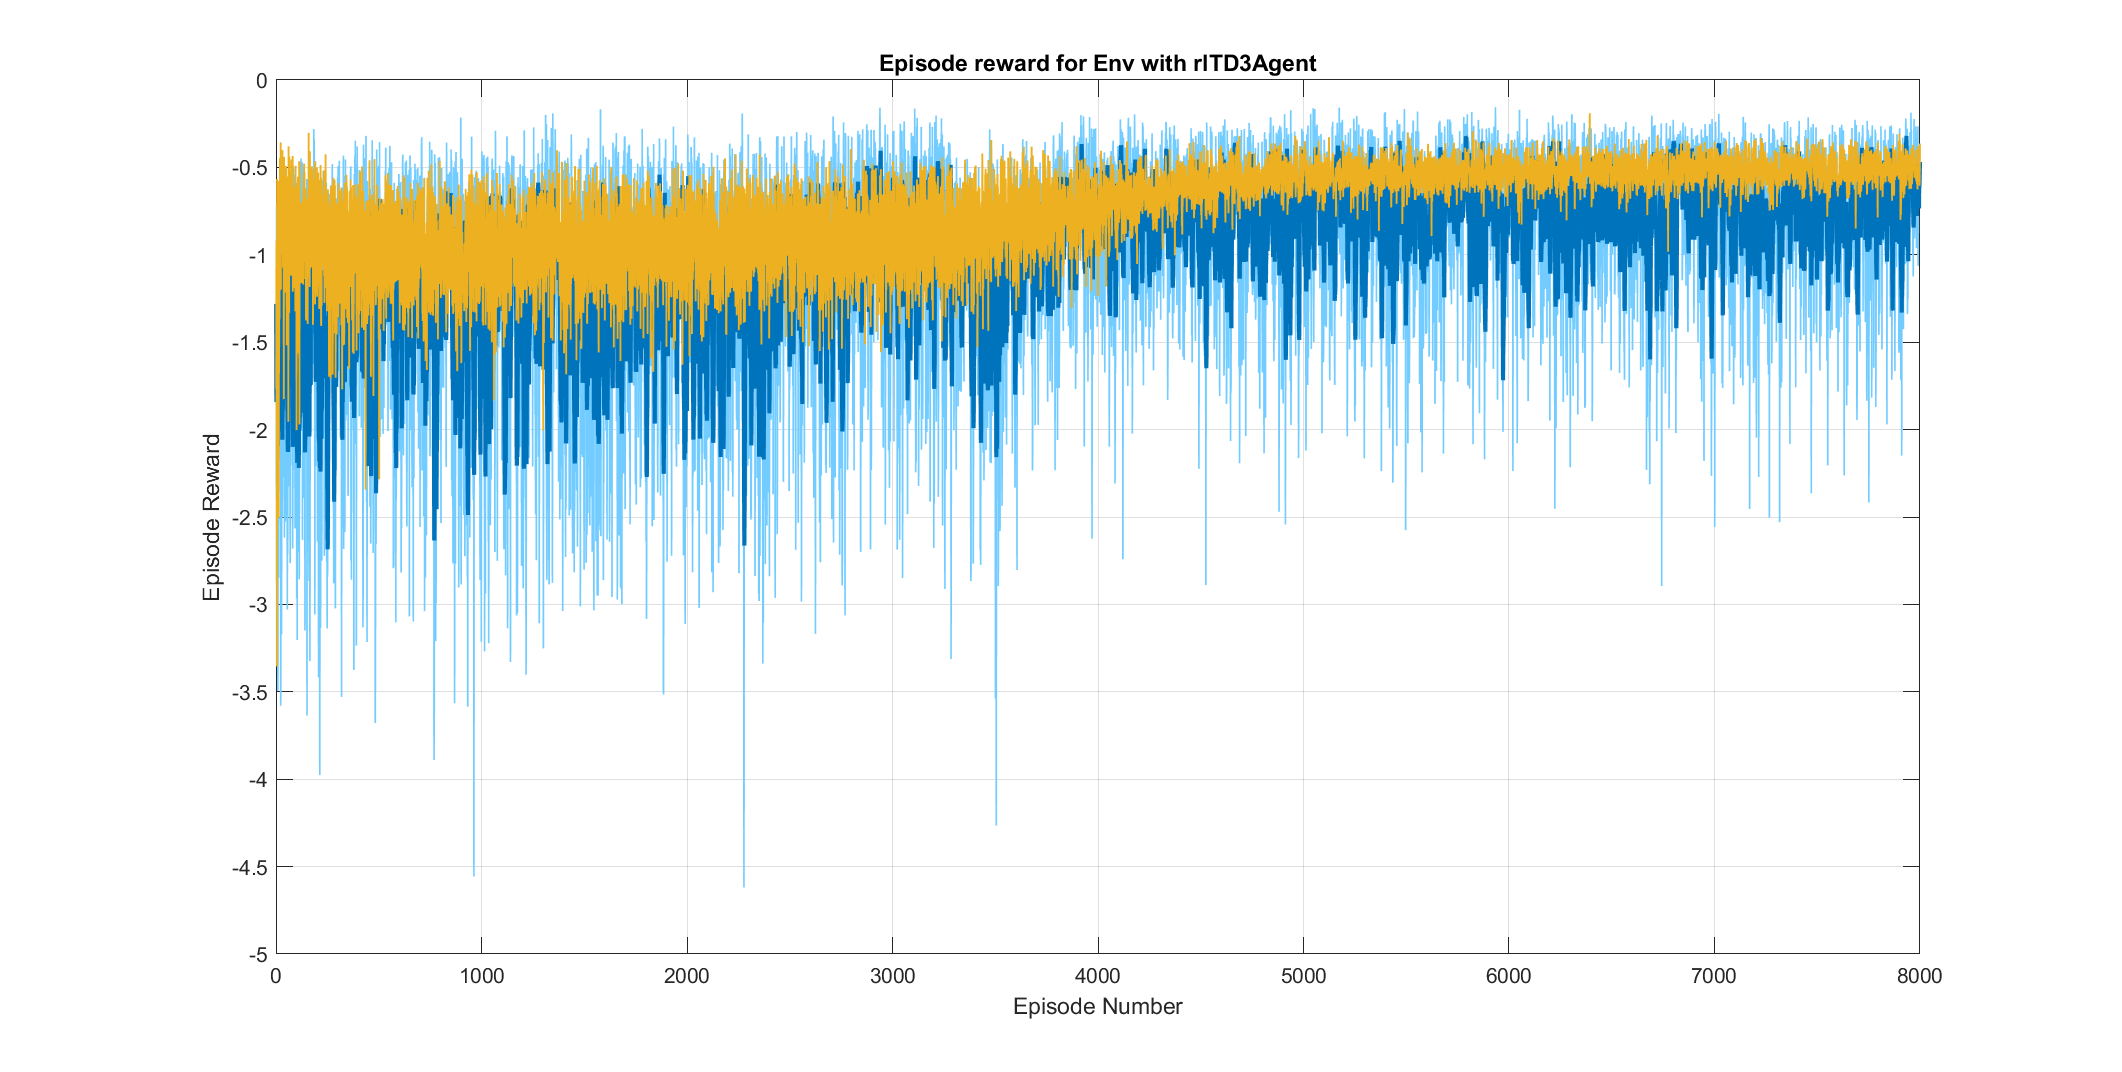
\includegraphics[width=\textwidth]{figures/training_progress_8000eps_valid_baseline.png}
\caption{Corrida larga v\'alida de 8000 episodios. La mejora contin\'ua hasta la zona final del entrenamiento.}
\end{figure}
}{}

\IfFileExists{figures/test_episode_49_valid_baseline_8000.png}{
\begin{figure}[H]
\centering
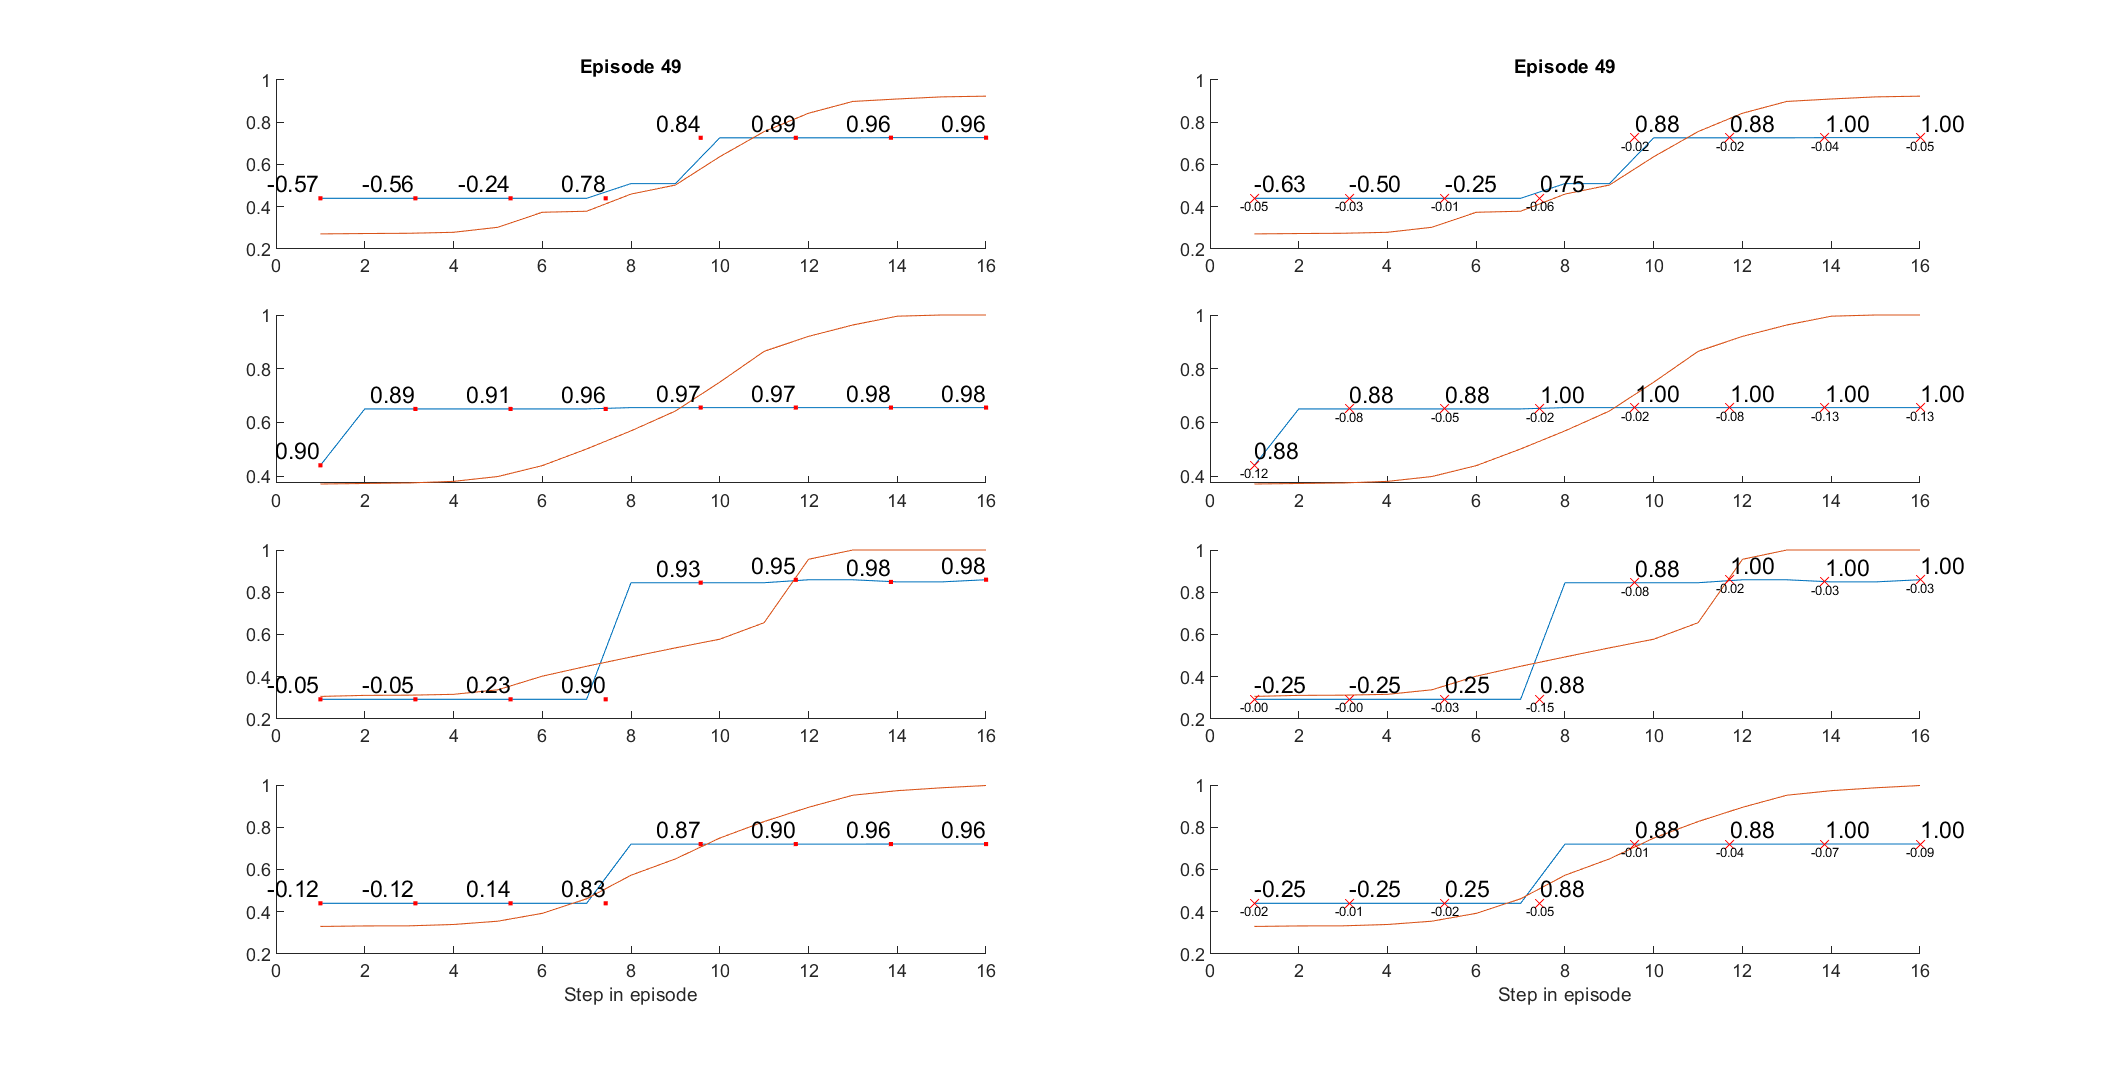
\includegraphics[width=\textwidth]{figures/test_episode_49_valid_baseline_8000.png}
\caption{Episodio 49 del test con \texttt{Agent7250}. La pr\'otesis sigue la referencia de forma claramente mejor que en el baseline inicial v\'alido.}
\end{figure}
}{}

M\'etricas del test final de 50 simulaciones con \texttt{Agent7250}:
\begin{itemize}[leftmargin=1.2cm]
    \item \texttt{trackingMSE = 0.043045},
    \item \texttt{trackingMAE = 0.160336},
    \item \texttt{actionL2 = 0.596444},
    \item \texttt{saturationFraction = 0.392086},
    \item \(\Delta a\) L2 \(= 0.321385\),
    \item \texttt{|PWM| medio = 178.288566}.
\end{itemize}

\subsection{Por qu\'e este resultado es importante}

Porque mejora simult\'aneamente varias cosas:
\begin{itemize}[leftmargin=1.2cm]
    \item menor error de tracking;
    \item menor error absoluto;
    \item menor energ\'ia total;
    \item menor saturaci\'on;
    \item mucha menor brusquedad.
\end{itemize}

Eso significa que el proyecto ya no solo aprende. Aprende de una forma mejor coordinada.

\section{Qu\'e ense\~na hoy este proyecto}

Si alguien quisiera resumir el aprendizaje t\'ecnico de todo el proyecto en pocas ideas, ser\'ian estas:
\begin{enumerate}[leftmargin=1.2cm]
    \item en problemas de RL para rob\'otica, una reward aparentemente razonable puede estar mal alineada;
    \item el \emph{logging} correcto es tan importante como el entrenamiento mismo;
    \item una acci\'on continua debe alinearse con la acci\'on f\'isica efectiva;
    \item si el simulador est\'a mal, las conclusiones sobre la policy tambi\'en quedan mal;
    \item una vez corregido el entorno, TD3 s\'i puede resolver el tracking de forma convincente en simulaci\'on.
\end{enumerate}

\section{Qu\'e sigue ahora}

El proyecto ya tiene un baseline serio. Por eso la siguiente fase no deber\'ia volver a cambiar demasiadas cosas a la vez. Lo m\'as sensato ahora es:
\begin{itemize}[leftmargin=1.2cm]
    \item mantener TD3;
    \item mantener el estado Markoviano de 52D;
    \item mantener la reward actual como punto de partida;
    \item estudiar c\'omo reducir a\'un m\'as saturaci\'on y esfuerzo sin perder tracking.
\end{itemize}

En otras palabras, la pregunta ya no es \emph{si el sistema puede aprender}.  
La pregunta correcta ahora es: \emph{c\'omo hacer que el control sea igual de preciso, pero m\'as fino y menos agresivo}.

\section{Conclusi\'on}

Esta gu\'ia deja una idea central muy clara: el proyecto no avanz\'o por una sola gran idea, sino por una secuencia de correcciones bien razonadas. Primero se entendi\'o el problema base. Despu\'es se audit\'o el reward. Luego se pas\'o a una formulaci\'on m\'as limpia con MSE. M\'as tarde se aline\'o la acci\'on aprendida con la acci\'on efectiva. Finalmente, se descubri\'o y corrigi\'o el bug del simulador, que era el cuello de botella m\'as serio.

El resultado de esa historia es el baseline actual con \texttt{Agent7250}: un agente que, en simulaci\'on, sigue la referencia de manera mucho mejor que al inicio del proyecto y lo hace adem\'as con menos brusquedad que el baseline v\'alido inicial.

Ese es el mejor punto posible para seguir aprendiendo y mejorando.

\bibliographystyle{plainnat}
\bibliography{references}

\end{document}
